\chapter{Project Functions}
\label{vl:tc-project}

[Project methodologies. Level of technical maturity - ProtoDUNE!.]

As defined in the \dword{dune} Management Plan (DMP), the \dword{dune}
\dword{tcoord} generates and recommends technical decisions to the
\dword{dune} collaboration \dword{exb}.
It consists of all consortia scientific and technical leads. It meets
on a regular basis (approximately monthly) to review and resolve
technical issues associated with detector construction. It reports
through the \dword{exb} to collaboration management. The \dword{dune} \dword{tb}
is chaired by the \dword{dune} \dword{tcoord}. The
\dword{tc} engineering team meets on a regular basis (approximately weekly)
to discuss more detailed technical issues. \Dword{tc} does not have
responsibility for financial issues; these are referred to
the \dword{exb} and Resource Coordinator (RC).

\Dword{tc} has several major project support tasks to accomplish:
\begin{itemize}
\item Assure that each consortium has a well defined and complete
  scope, that the interfaces between the consortia are sufficiently
  well defined and that any remaining scope can be covered by \dword{tc}
  through \dword{comfund} or flagged as missing scope to the EB and RC. In
  other words, assure that the full detector scope is
  identified. Monitor the interfaces and consortia progress in
  delivering their scope.
\item Develop an overall project \dlong{ims}
  that includes reasonable production schedules, testing plans and a
  well developed installation schedule from each consortium. Monitor
  the \dword{ims} as well as the individual consortium schedules.
\item Ensure that appropriate engineering and safety standards are
  developed and agreed to by all key stakeholders and that these
  standards are conveyed to and understood by each
  consortium. Monitor the design and engineering work.
\item Ensure that all \dword{dune} requirements on \dword{lbnf} for
  conventional facilities, cryostat and cryogenics have been clearly
  defined and understood by each consortium. Negotiate scope
  boundaries with \dword{lbnf}. Monitor \dword{lbnf} progress on
  final conventional facility design, cryostat design and cryogenics
  design.
\item Ensure that all technical issues associated with scaling from
  \dword{protodune} have sufficient resources to converge on
  decisions that enable the detector to be fully integrated and
  installed.
\item Ensure that the integration and \dword{qc} processes for each
  consortium are fully developed and reviewed and that the
  requirements on an \dword{itf} are well defined.
\end{itemize}

\Dword{tc} is responsible for technical quality and schedule and is not
responsible for consortia funding or budgets.  \Dword{tc} will try to help
resolve any issue that it can, but will likely have to push all
financial issues to the TB, EB and RC for resolution.

\Dword{tc} maintains a web
page\footnote{\url{https://web.fnal.gov/collaboration/DUNE/DUNE\%20Project/\_layouts/15/start.aspx\#/}.}
with links to project documents. \Dword{tc} maintains repositories of
project documents and drawings. These include the \dword{wbs},
schedule, risk register, requirements, milestones, strategy, detector
models and drawings that define the \dword{dune} detector.

%%%%%%%%%%%%%%%%%%%%%%%%%%%%%%%%
\section{WBS}
\label{sec:fdsp-coord-wbs}

The DUNE WBS at level 1 includes six categories as shown in
Fig.~\ref{fig:WBS_level2}.
\begin{dunefigure}[DUNE WBS at level 2]{fig:WBS_level2}
  {High level DUNE WBS to level 2.}
  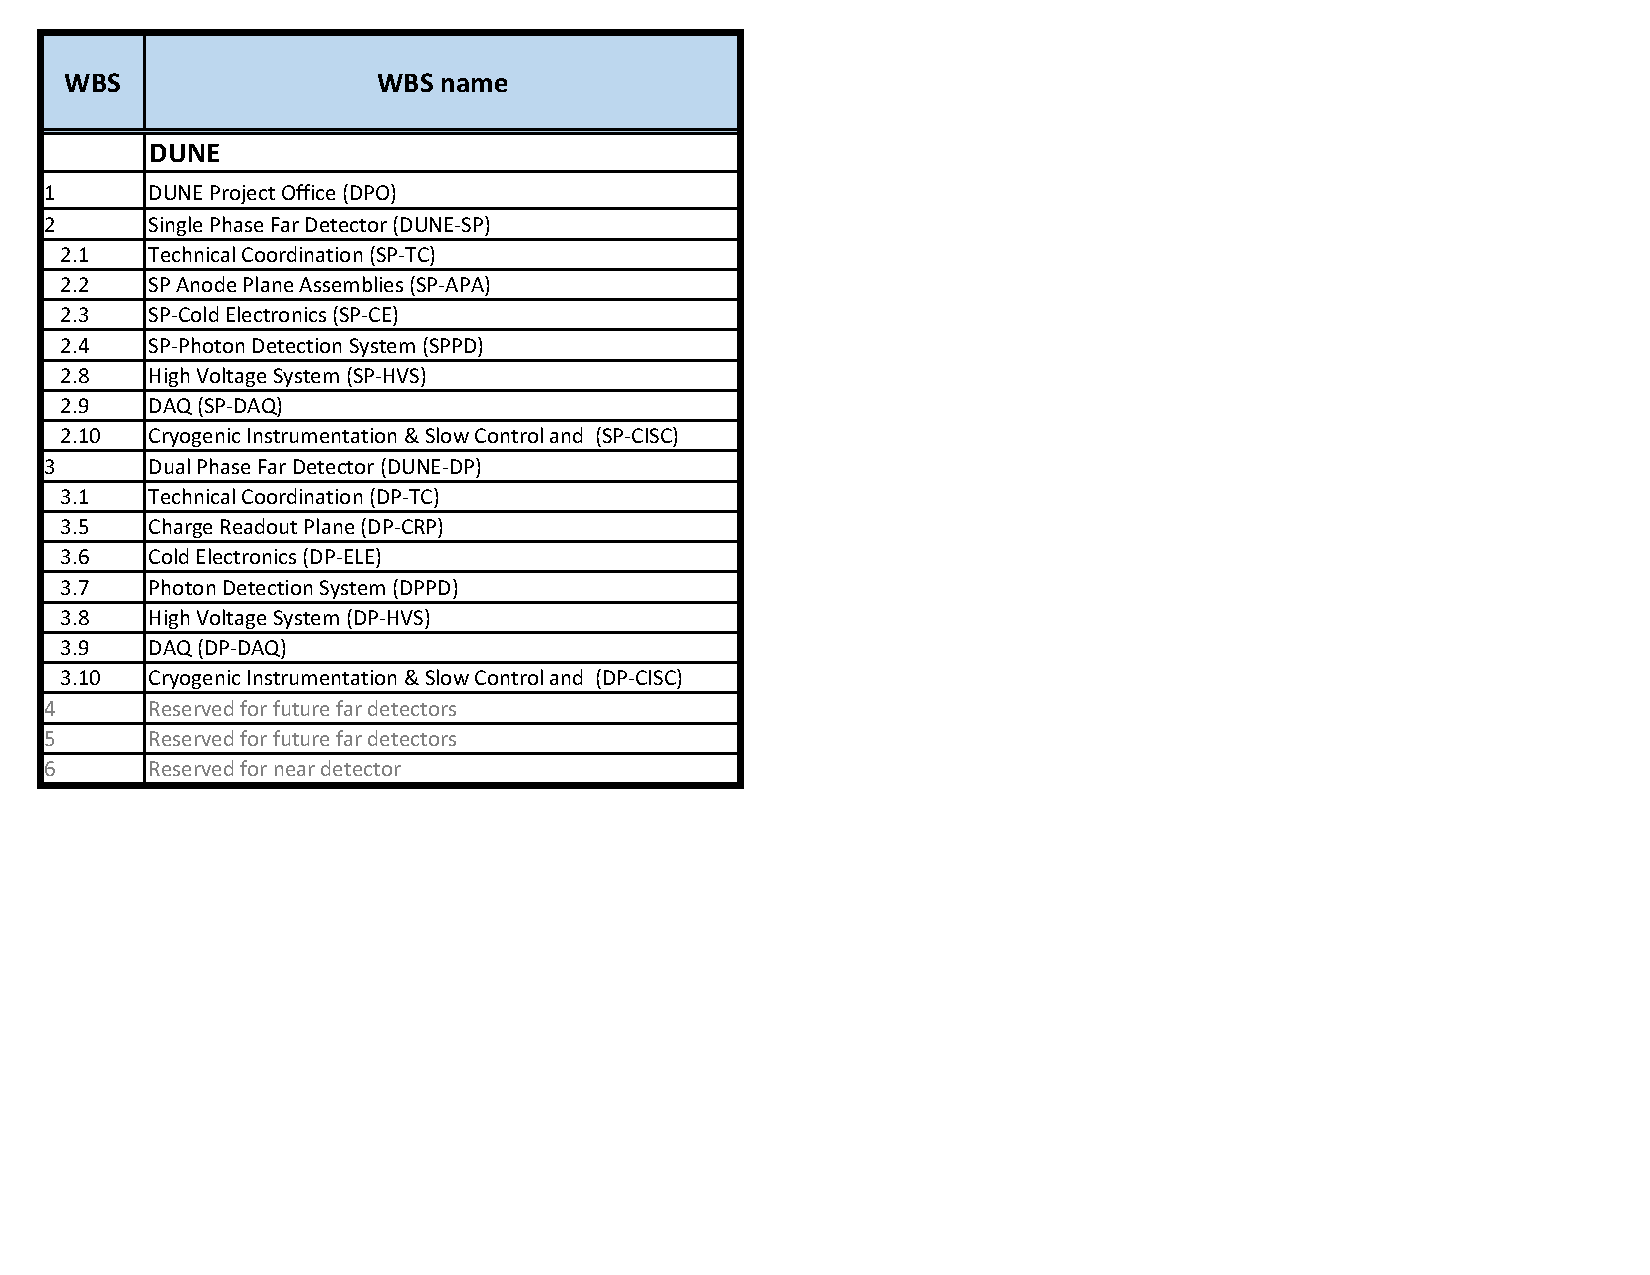
\includegraphics[width=0.75\textwidth]{WBS_level2}
\end{dunefigure}
At level 2 the WBS has a breakdown of seven items
each for single-phase and dual-phase far detectors.

Each subsystem WBS is owned by the associated consortium. They follow a common format with the first level (level 3) broken down in rough time sequence with the following categories:
\begin{enumerate}
  \item Management
  \item Physics and Simulation
  \item Design, Engineering, and R\&D
  \item Production Setup
  \item Production
  \item Integration (ITF)
  \item Installation (SURF)
\end{enumerate}
Subsequent levels in the WBS generally follow consortia subsystem structure.
This WBS has been used as the framework to capture all of the costs
for the overall DUNE project cost estimate.

%%%%%%%%%%%%%%%%%%%%%%%%%%%%%%%%
\section{Cost}
\label{sec:fdsp-coord-cost}

A preliminary total DUNE project cost estimate based on ProtoDUNE
costs was provided to the Neutrino Cost Group in August 2018. Based on
feedback from that review and updated cost estimates based on DUNE
designs, an updated cost estimate has been developed. A corresponding
project schedule has been developed and is discussed in
Section~\ref{sec:fdsp-coord-controls}.

The cost estimate includes the materials and services (M\&S) cost in
local currencies in 2018, converted to 2018 US\$. The cost estimate
includes the number of labor hours broken down into eight categories
(engineer, designer, technician, student, postdoc, graduate student,
scientist, faculty). There is no escalation included in the cost estimate.

The cost estimate is for one single-phase and one dual-phase far
detector, where the sequencing assumes that the single-phase detector
comes first. This implies that some common costs are captured in the
single-phase cost estimate.

No operations costs are included. While some parts of the detector are
accessible and equpment can be maintained, other parts are not. For
those systems with accessible equipment some costs are included for
replacement over the life of the detector.

\begin{itemize}
 \item cost model, how many SP/DP detectors
 \item spares, labor categories, ...
 \item summary of consortia costs
 \item TC cost details?
\end{itemize}

%%%%%%%%%%%%%%%%%%%%%%%%%%%%%%%%
\section{MOU}
\label{sec:fdsp-coord-mou}

Memoranda of Understanding (MOU) with each group collaborating in a
consortium will be held by DUNE/FNAL?

%%%%%%%%%%%%%%%%%%%%%%%%%%%%%%%%
\section{Budget}
\label{sec:fdsp-coord-budget}

\dword{dune} \dword{tc} will be supported by \dword{comfund} and host
country. The \dword{comfund} is overseen by the Resource Coordinator. The
host country contribution is through a \dword{tc}
Operations Budget from DOE and managed by the \dword{tcoord}.

%%%%%%%%%%%%%%%%%%%%%%%%%%%%%%%%
\section{Schedule}
\label{sec:fdsp-coord-controls}

A series of tiered milestones have been developed for the \dword{dune}
project. The Tier-0 milestones are held by the spokespersons and host
laboratory director. Three have been defined and the current milestones and
dates are:
\begin{enumerate}
\item Start main cavern excavation \hspace{2.58in} 2019
\item Start \dword{detmodule}~1 installation \hspace{2.1in} 2022
\item Start operations of \dword{detmodule}~1--2 with beam \hspace{1in} 2026
\end{enumerate}
These dates will be revisited at the time of the \dword{tdr} review.  Tier-1
milestones will be held by the technical coordinator and \dword{lbnf} Project
Manager and will be defined in advance of the \dword{tdr} review. Tier-2
milestones will be held by the consortia.

A high level version of the \dword{dune} milestones from the \dword{ims}
can be seen in Table~\ref{tab:DUNE_schedule}.
\begin{dunetable}
  [Overall \dword{dune} Project Tier-1 milestones.]
  {p{0.84\linewidth}p{0.14\linewidth}}
  {tab:DUNE_schedule}
  {Overall \dword{dune} Project Tier-1 milestones.}
  Milestone & Date   \\ \toprowrule
  RRB Approval of Technical Design Review                       & 09/02/2019 \\ \colhline
  Beneficial Occupancy of Integration Test Facility             & 09/01/2021 \\ \colhline
  Construction of steel frame for Cryostat \#1 complete         & 12/17/2021 \\ \colhline
  Construction of Mezzanine for Cryostat \#1 complete           & 01/17/2022 \\ \colhline
  Begin integration/testing of Detector \#1 components at ITF   & 02/01/2022 \\ \colhline
  Beneficial Occupancy of Central Utility Cavern Counting room  & 04/16/2022 \\ \colhline
  Construction of steel frame for Cryostat \#2 complete         & 07/01/2022 \\ \colhline
  Construction of Mezzanine for Cryostat \#2 complete           & 08/01/2022 \\ \colhline
  \textbf{Beneficial occupancy of Cryostat \#1}                 & \textbf{12/23/2022} \\ \colhline
  Cryostat \#1 ready for TPC installation                       & 05/01/2023 \\ \colhline
  Begin integration/testing of Detector \#2 components at ITF   & 11/01/2023 \\ \colhline
  \textbf{Beneficial occupancy of Cryostat \#2}                 & \textbf{03/01/2024} \\ \colhline
  Begin closing Temporary Construction Opening for Cryostat \#1 & 05/01/2024 \\ \colhline
  Cryostat \#2 ready for TPC installation                       & 08/01/2024 \\ \colhline
  Cryostat \#1 ready for filling                                & 10/01/2024 \\ \colhline
  Begin closing Temporary Construction Opening for Cryostat \#2 & 07/18/2025 \\ \colhline
  \textbf{Detector \#1 ready for operations}                    & \textbf{10/01/2025} \\ \colhline
  Cryostat \#2 ready for filling                                & 12/05/2025 \\ \colhline
  \textbf{Detector \#2 ready for operations}                    & \textbf{12/18/2026} \\
\end{dunetable}

\Dword{tc} will maintain the \dword{ims} that links all consortium schedules
and contains appropriate milestones to monitor progress.
It is currently envisioned as
three levels of control and notification milestones in addition to the
detailed consortium schedules. The highest level contains external
milestones, with the second level containing the key milestones for \dword{tc}
to monitor deliverables and installation progress, and the third level
containing the inter-consortium links. The schedules will go
under change control after agreement with each consortium on the
notification milestone dates and the \dword{tdr} is approved.

In addition to the overall \dword{ims} for construction and
installation, a schedule of key consortia activity in the period
2018--19  has been developed.

To ensure that the \dword{dune} detector remains on schedule,
\dword{tc} will monitor schedule statusing from each consortium, will organize
reviews of schedules and risks as appropriate.  As schedule problems
arise \dword{tc} will work with the affected consortium to resolve the
problems. If problems cannot be solved, \dword{tc} will take the issue to the
\dword{tb} and \dword{exb}.

A monthly report with input from all consortia will be published by
\dword{tc}. This will include updates on consortium technical progress and
updates from \dword{tc} itself.

%%%%%%%%%%%%%%%%%%%%%%%%%%%%%%%%
\section{Risks}
\label{sec:fdsp-coord-risks}

\dword{dune} has implemented a risk registry in
DocDB-6443. This document includes tabs for consortia risks
and \dword{tc}. It includes a tab for the overall
\dword{dune} risks. The overall \dword{dune} risks are shown in
Tables~\ref{fig:dune_risks1} and~\ref{fig:dune_risks2}. This registry
is currently being updated on an approximately annual basis.
\begin{dunefigure}[DUNE overall risk register]{fig:dune_risks1}
  {First page of DUNE overall risk register.}
  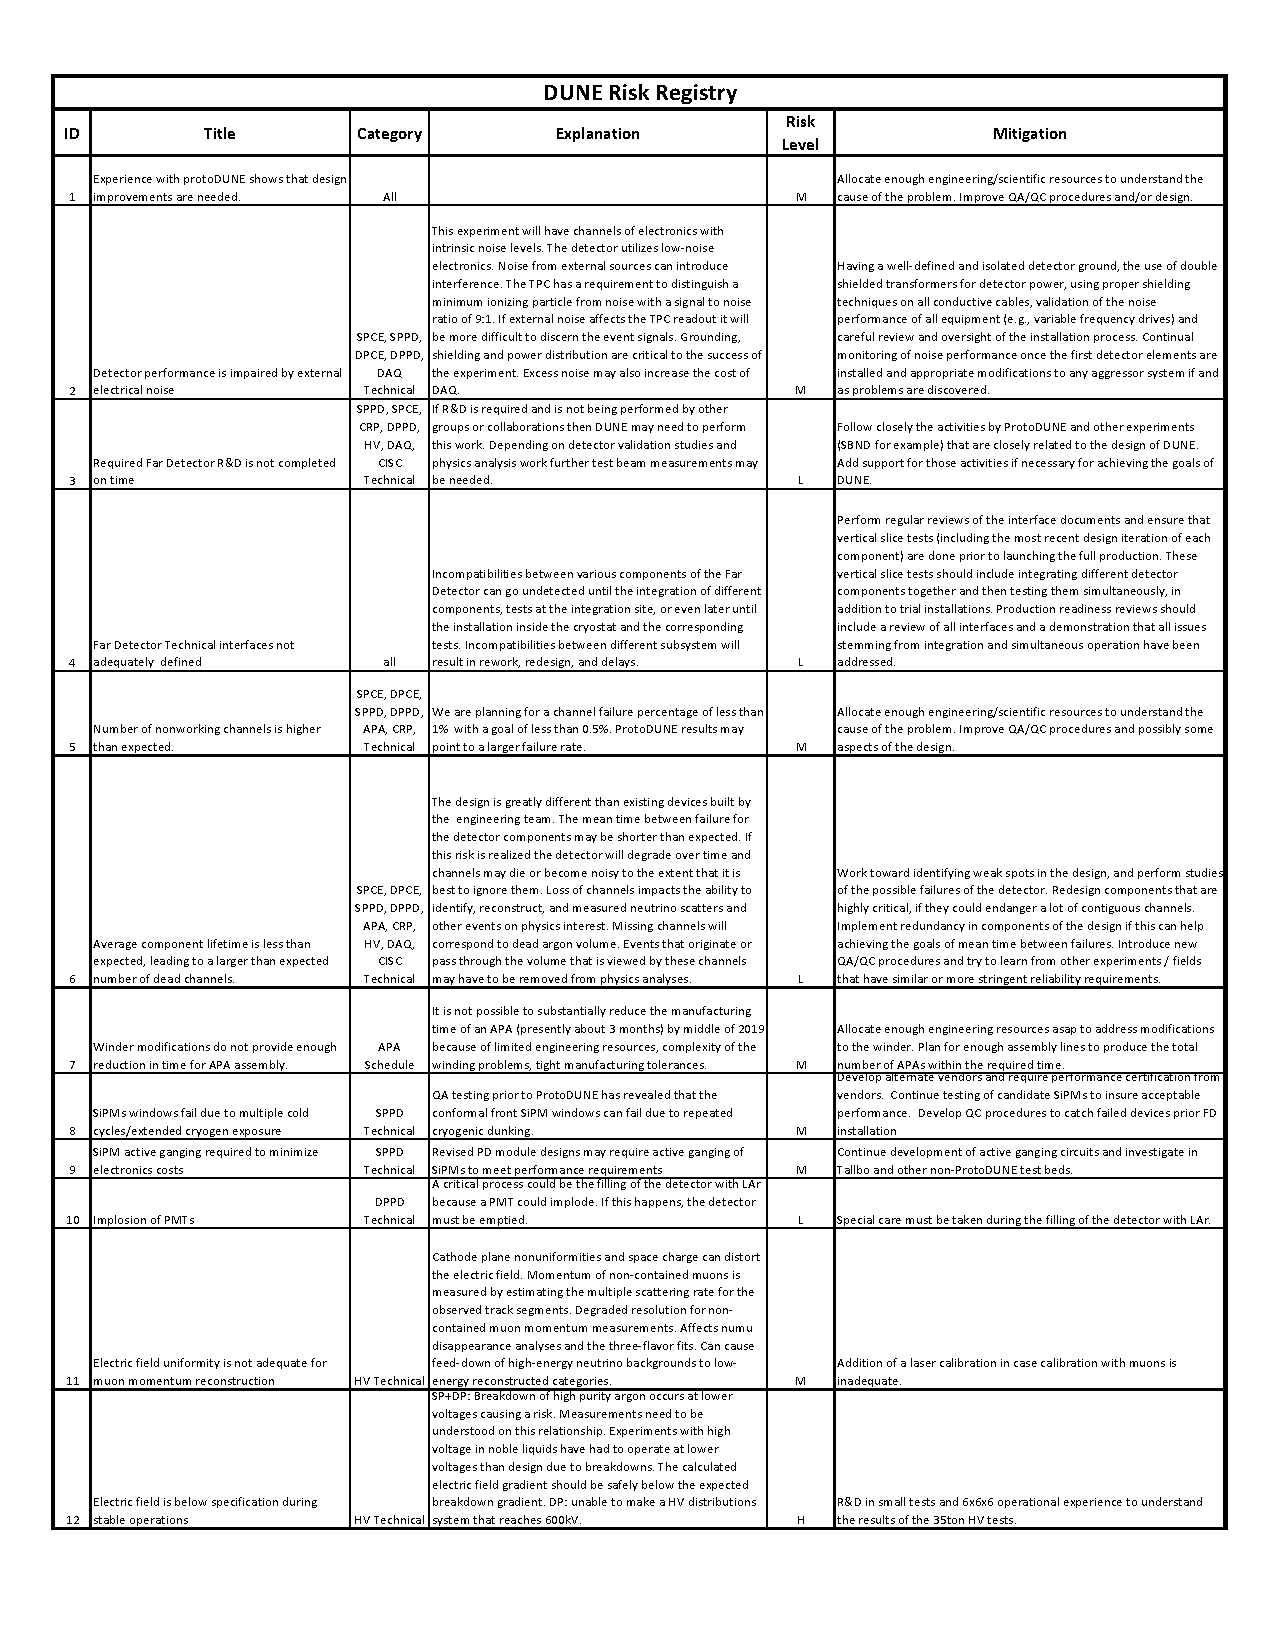
\includegraphics[width=0.95\textwidth]{DUNE_Risks_v4a1}
\end{dunefigure}
\begin{dunefigure}[DUNE overall risk register]{fig:dune_risks2}
  {Second page of DUNE overall risk register.}
  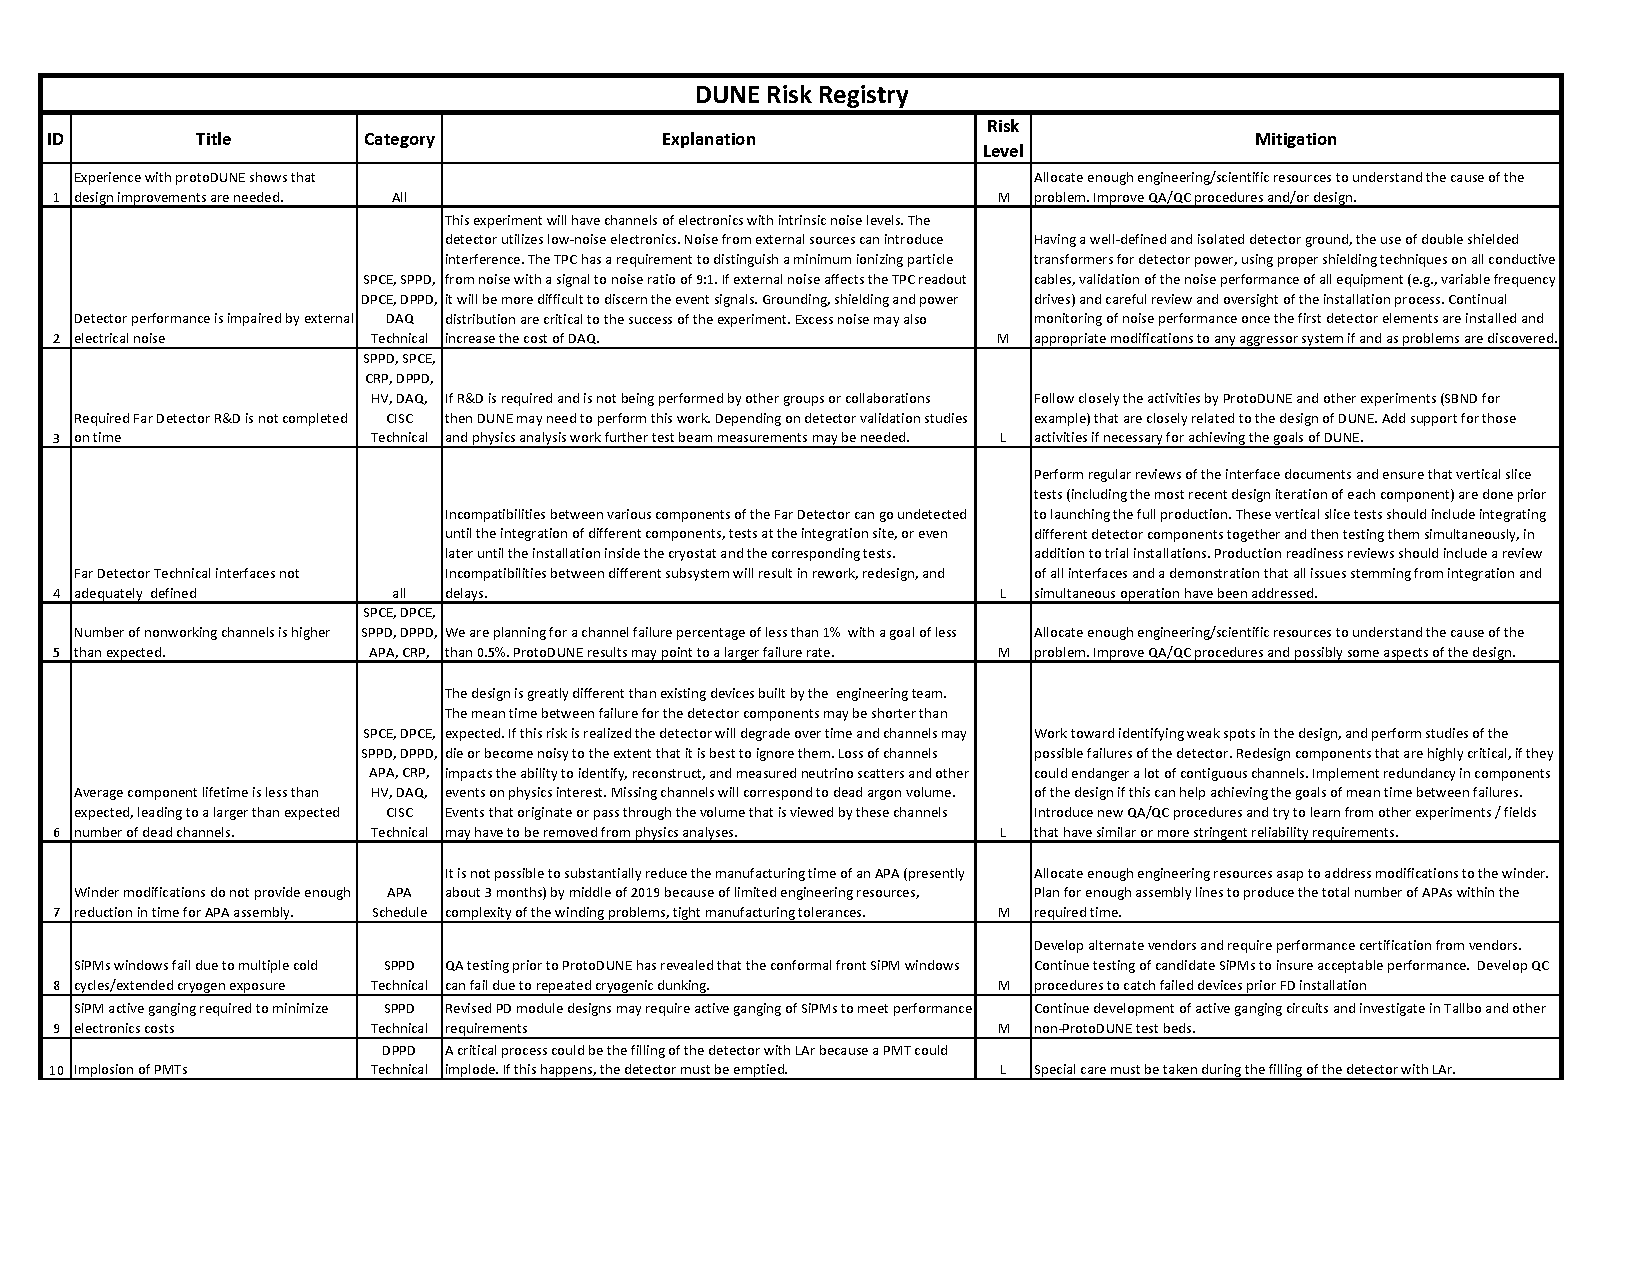
\includegraphics[width=0.95\textwidth]{DUNE_Risks_v4a2}
\end{dunefigure}
\dword{lbnf} and \dword{dune}-US would like \dword{dune} to update and
expand this risk register to enable a monte carlo analysis of cost and
schedule risks to the US project resulting from the international
\dword{dune} risks. This request is under consideration.

The \dword{tc} risks are summarized in Table~\ref{fig:tc_risks}.
\begin{dunefigure}[\dword{tc} risks]{fig:tc_risks}
  {\dword{tc} risk register.}
  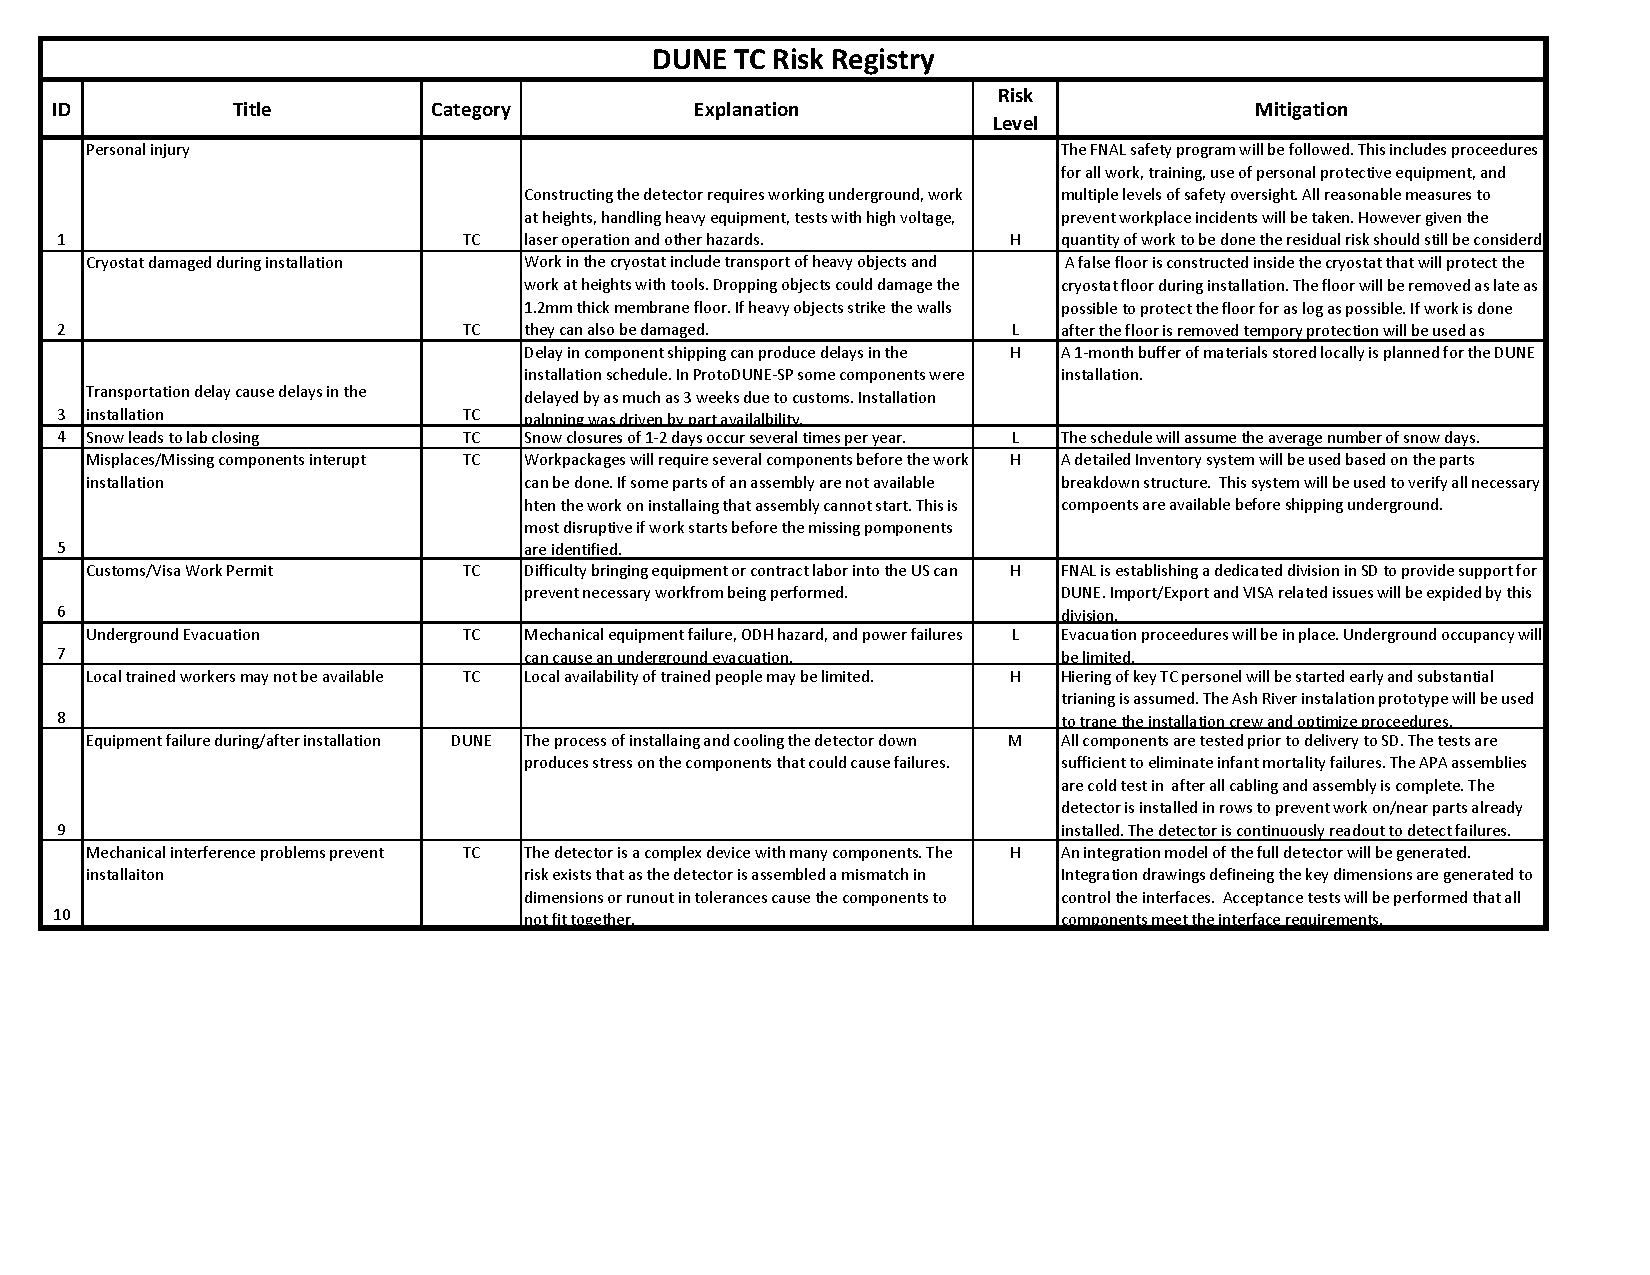
\includegraphics[width=0.9\textwidth]{TC_Risks_v4a}
\end{dunefigure}


The successful operation of \dword{protodune} retires many
potential risks to \dword{dune}. This includes most risks associated with the
technical design, production processes, \dword{qa}, integration
and installation. Residual risks remain relating to design and
production modifications associated with scaling to \dword{dune}, mitigations
to known installation and performance issues in \dword{protodune}, underground
installation at \surf and organizational growth.

The highest technical risks include: development of a system to
deliver \SI{600}{kV} to the \dual cathode; general delivery of the
required \dword{hv}; cathode and \dword{fc} discharge to the cryostat
membrane; noise levels, particularly for the \dword{ce}; %cold TPC electronics,
number of dead channels; lifetime of components surpassing \dunelifetime{}; %20 years,
\dword{qc} of all components; verification of improved \dword{lem}
performance; verification of new cold  \dword{adc} and  \dword{coldata} performance;
argon purity; electron drift lifetime; \phel light yield;
incomplete calibration plan; and incomplete connection of design to
physics. Other major risks include insufficient funding, optimistic
production schedules, incomplete integration, testing and installation
plans.

Key risks for \dword{tc} to manage include the following:
\begin{enumerate}
\item Too much scope is unaccounted for by the consortia and falls
  to \dword{tc} and \dword{comfund}.
\item Insufficient organizational systems are put into place to
  ensure that this complex international mega-science project,
  including \dword{tc}, \fnal as host laboratory, \surf, DOE and all international
  partners continue to successfully work together to ensure
  appropriate rules and services are provided to enable success of
  the project.
\item Inability of \dword{tc} to obtain sufficient personnel resources so as to
  ensure that \dword{tc} can oversee and coordinate all of its
  project tasks.  While the USA has a special responsibility towards
  \dword{tc} as host country, it is expected that personnel resources will
  be directed to \dword{tc} from each collaborating country. Related to this
  risk is the fact that consortium deliverables are not really
  stand-alone subsystems; they are all parts of a single \dword{detmodule}. This
  elevates the requirements on coordination between consortia.
\end{enumerate}

The consortia have provided preliminary versions of risk analyses that
have been collected on the \dword{tc} webpage. These are being developed into
an overall risk register that will be monitored and maintained by \dword{tc}
in coordination with the consortia.

%%%%%%%%%%%%%%%%%%%%%%%%%%%%%%%%
\section{Requirements}
\label{sec:fdsp-coord-requirements}

\dword{dune} scientific goals as described in the TDR Executive Summary\ref{tdr:exec_sum} include:
\begin{itemize}
\item a comprehensive program of neutrino oscillation measurements including the search for CP violation
\item measure $\nu_{e}$ flux from a core-collapse supernova within our galaxy should one occur during DUNE operations
\item search for baryon number violation
\end{itemize}
These goals motivate a number of key detector requirements: drift
field, electron lifetime, system noise, photon detector light yield,
and event time resolution. The \dword{exb} has approved a list of high
level detector specifcations, including those listed above. These are
maintained in edms-xxxx and are highlighted in
Table~\ref{tab:dunephysicsreqs}.
\begin{dunetable}
  [DUNE requirements owned by \dword{exb}]
  {p{0.025\textwidth}p{0.05\textwidth}p{0.2\textwidth}p{0.35\textwidth}p{0.15\textwidth}p{0.1\textwidth}}
  {tab:dunephysicsreqs}
  {\dword{dune} high level system requirements owned by \dword{exb}}
  ID & System & Parameter & Physics Requirement Driver & Requirement & Goal \\ \toprowrule
  1   & HVS    & Minimum drift field &  Limit recombination, diffusion and space charge impacts on $e$, $\mu$, $p$ particle ID. Establish constant drift velocity and adequate \dword{s/n} on induction planes for tracking. & >\SI{250}{V/cm} & \spmaxfield \\ \colhline
  2   & CE     & System noise & The noise specification is driven by pattern recognition and two-track separation.  Studies suggest that a minimum of ~5/1 signal to noise ratio on individual wire measurements allows for sufficient reconstruction performance. Converting this signal to noise ratio to ENC on an induction plane singal for a MIP with minimum signal yields the figure of system-noise. The corresponding ratio on the collection wires is ~13/1.  & <\SI{1000}{enc} & ALARA \\ \colhline
  3   & PDS    & Light yield  & The light yield shall be sufficient for measuring event time (and total intensity) of events with visible energy above 200 MeV.  Goal is to make possible a 10\% energy measurement for events with a visible energy of 10 MeV.  & >\SI{0.5}{pe/MeV} & >\SI{5}{pe/MeV}  \\ \colhline
  4   &        &   &   & &  \\ \colhline
\end{dunetable}

The high level \dword{dune} requirments that drive the \dword{lbnf} design are
maintained in DocDB-112 and under change control. These are owned by
the \dword{dune} \dword{tc} and the \dword{lbnf} project manager.

\begin{itemize}
 \item Summary of consortia requirements?
 \item TC requirements (cleanliness, APA spacing, ...)?
\end{itemize}


%%%%%%%%%%%%%%%%%%%%%%%%%%%%%%%%
\section{Value Engineering}
\label{sec:fdsp-coord-ve}

Value engineering is an ongoing process to arrive at cost effective solutions to the technical challenges of building the \dword{dune} detector.
This process is executed at both the consortia and \dword{tc} level.

%%%%%%%%%%%%%%%%%%%%%%%%%%%%%%%%
\section{Lessons Learned}
\label{sec:fdsp-coord-lessons}

A detailed list of lessons learned from the construction and operation
of ProtoDUNE-SP has been compiled in DocDB-8255. These lessons have driven the
planning for DUNE and have led to design changes for DUNE.

%%%%%%%%%%%%%%%%%%%%%%%%%%%%%%%%
\section{Interface to National Projects}
\label{sec:fdsp-coord-national}

\dword{dune} \dword{tc} works with each consortia leadership team. The
consortia leadership team consists of the consortia lead and the
consortia technical lead and others appointed by the consortia
lead. The consortia leadership teams usually contain representatives
of the various national projects that provide the funding to build the consortia
deliverables. If the consortia leadership teams are not directly
embedded in the various national projects building their subsystem,
then the consortia leadership teams represent their national projects
to \dword{tc}. The consortia leadership teams are responsible for
providing their deliverables on time according to the
\dword{ims}. They are responsible for identifying any inconsistencies
between the \dword{ims} and their national project schedules and
bringing these issues to \dword{tc}. The consortia leadership teams
are responsible for reporting progress against the \dword{ims} to
\dword{tc}.

%%%%%%%%%%%%%%%%%%%%%%%%%%%%%%%%
\section{Reporting}
\label{sec:fdsp-coord-reporting}

The \dword{dune} project has been providing regular monthly reports
since the ramp up of ProtoDUNE in summer 2016. The project plans to
continue these reports into the future. Reporting will expand to
include monthly reports against the \dword{ims}.

The \dword{dune} project provides regular reports to LBNC reviews
several times a year.

The \dword{dune} project produces reports from design, production and operations reviews.

%%%%%%%%%%%%%%%%%%%%%%%%%%%%%%%%
%\section{Management of Schedule and Risks}
%\label{sec:fdsp-coord-mgmt}


%%%%%%%%%%%%%%%%%%%%%%%%%%%%%%%%
\section{Design Process}
\label{sec:fdsp-coord-designprocess}

The design process follows the engineering safety process and review
processes described in Chapter~\ref{vl:tc-review}.

%%%%%%%%%%%%%%%%%%%%%%%%%%%%%%%%
\section{Integration Facility}
\label{sec:fdsp-coord-itf}

Do we explain the concept of ITF here in general terms? May be better
in Chapter~\ref{vl:tc-facility}?
